\documentclass[12pt]{article}
\usepackage[left=1in,headheight=48pt]{geometry}
\usepackage{graphicx}
\graphicspath{{images/}}
\usepackage{wrapfig}
\usepackage{comment}
\usepackage{listings}
\usepackage{xcolor}
\usepackage{float}
\usepackage{biblatex}
\addbibresource{fish.bib}
 
\definecolor{codegreen}{rgb}{0,0.6,0}
\definecolor{codegray}{rgb}{0.5,0.5,0.5}
\definecolor{codepurple}{rgb}{0.58,0,0.82}
\definecolor{backcolour}{rgb}{0.95,0.95,0.92}
 
\lstdefinestyle{mystyle}{
    backgroundcolor=\color{backcolour},
    commentstyle=\color{codegreen},
    keywordstyle=\color{magenta},
    numberstyle=\tiny\color{codegray},
    stringstyle=\color{codepurple},
    basicstyle=\fontsize{10}{12}\ttfamily,
    breakatwhitespace=false,
    breaklines=true,
    %breaklines=false,
    captionpos=b,
    keepspaces=true,
    numbers=left,
    numbersep=5pt,
    showspaces=false,
    showstringspaces=false,
    showtabs=false,
    tabsize=2
}
 
\lstset{style=mystyle}

\title{Report for End of Year on Progress on Fish Tracking Software}
\author{Ari Spraggins}
\date{2020-11-19}

\begin{document}

\maketitle
\abstract{One of the major problem encountered when using the positions of fish in analysis is a tendency for the software to transpose the identities of the two fish whenever they cross. The goal of this program is to analyse that data and to remove that error from it. To do so we are comparing a metric that is unique to the fishes before and after the crossing, in this case a histogram of their brightness, and comparing them.}

\section{Introduction}

The basis of this work is going to be the videos of fish swimming in a tank, more specifically a video of 2 fish. In each frame we use software that identifies dark spots as the fish.

\textbf{\textit{Example picture of fish}}

\begin{figure}[H]
	\centering
	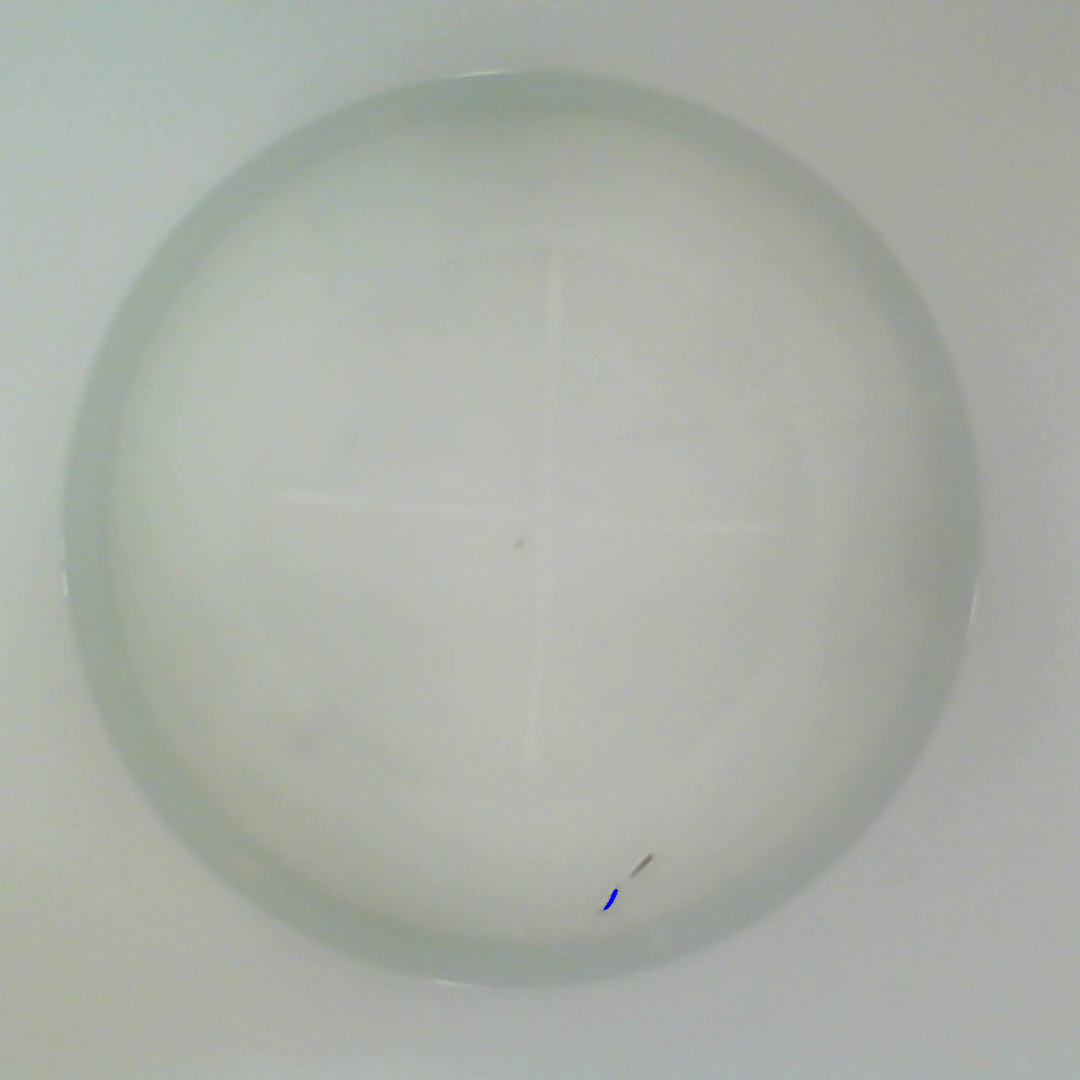
\includegraphics[width=.75\linewidth]{fish}
	\caption{The two fishes}
	\label{fig:fish}
\end{figure}

We can use this identified fish to compare how the fish has moved from frame to frame. Once we have the position of the fish in the next frame we have compare the change between two frames by using a matrix.

\textbf{\textit{Example picture of two frames}}

\begin{figure}[H]
	\centering
	\includegraphics[width=.75\linewidth]{fish2}
	\caption{The distance matrix}
	\label{fig:fish2}
\end{figure}

We can the extend this frame by frame comparison over the regions where the fish are visually distinct. However, in ranges where the positions of the fishes are reported as overlapping, this approach won't work for obvious reasons. 

\textbf{\textit{Example picture of crossing}}

Instead, during these ranges, we have to take the more involved approach of comparing a visually distinctive features of the fishes from frame. The easiest feature to compare is this case is the brightness of the fish, which we can compare via a histogram.

\textbf{\textit{Example Picture of histogram}}

\begin{figure}[H]
	\centering
	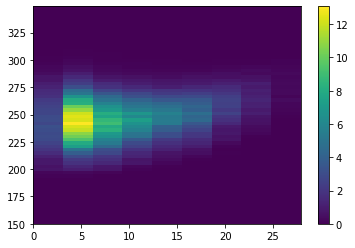
\includegraphics[width=.75\linewidth]{hist}
	\caption{The histogram}
	\label{fig:hist}
\end{figure}

%\section{Previous Work}

\section{Results}

What we are doing in essence is taking the images of the fish and comparing the from one point in time to the next. To do this we are taking the parts of the 

The 


\section{Methods}

One of the things that quickly becomes apparent is that the fish are present as a series of dark pixels against a white background, which means that we can feed the image of a frame to a different software (in this case trilab-tracker) to generate a list of pixels that compose the fishes for tracking. This software returns the fish as either a pair of arrays for the regions where it detects two fish, and a single array where it detects one fish of the form [frame][fish][xpixels, ypixels][color]. Once we have the fish in an array form for ease of operation, we can begin performing an initial unswap by tracking the distance between the fish to determine if there was a swap, by comparing the on and off axis distances of the two possible positions of the fish. The downside of this approach is that it only works in areas in which the tracker returns that there is two fish, so we will first need to determine what regions are overlapping and nonoverlapping. Once we have these nonoverlapping regions, we can begin performing the swap check. 

\begin{minipage}[c]{\textwidth}
\begin{lstlisting}[language=Python]
def swapStatus(pos,i):
    '''
    Detect swaps between consecutive frames based on proximity.
    
    Input:
        pos:Postionts. Array with shape (Nframes,Nfish,Ndimensions),
        i: Frame index. Int.
    
    Output:
        Int. 0 if no swaps, 1 if swapped, 2 if overlapping.
    '''
    nFish=pos.shape[1] #Number of fish
    distanceMatrix=[np.linalg.norm(pos[i+1][0]-pos[i][0]),
                    np.linalg.norm(pos[i+1][1]-pos[i][1]),
                    np.linalg.norm(pos[i+1][0]-pos[i][1]),
                    np.linalg.norm(pos[i+1][1]-pos[i][0])]
    swapCriteron=(distanceMatrix[0]+distanceMatrix[1])-(distanceMatrix[2]+distanceMatrix[3])
    if abs(swapCriteron)<1e-10:
        return 2 #Overlapping
    elif swapCriteron>0:
        return 1 #Swapped
    elif swapCriteron<0:
        return 0 #Normal
    else:
        return -1
\end{lstlisting}
\end{minipage}

Once we have this data for the nonoverlapping ranges, we have to switch approaches for the overlapping regions. Since we can't compare the distances with the software only reporting a single fish, we are forced to use a different technique., we are using the technique of comparing the histograms of the brightness of the fishes before and after an overlapping range, as proposed by the paper on idTracker\cite{idTracker}. The process for this is for us to feed the arrays directly into numpy's histogram2d, which allows us to compute the histograms with a minimal amount of effort other than determining the correct bins. After that we need to manipulate the data slightly so that the histograms are taken as the average over the nonoverlapping regions for more accuracy, and are then saved out for comparison.

\begin{minipage}[c]{\textwidth}
\begin{lstlisting}[language=Python]
for i in tnrange(60,desc='nonOverlappingRange'):
    for k in range(2):
        countSum=0
        countDif=0
        pairData=[]
        for j in range(*nonOverlappingRange[i]):
            fishPixels = fishU[j][k]
            m,l=np.triu_indices(fishPixels.shape[0],k=1)
            d=np.sqrt((fishPixels[l,0]-fishPixels[m,0])**2+(fishPixels[l,1]-fishPixels[m,1])**2)
            bSum=fishPixels[l,2]+fishPixels[m,2]
            bDif=fishPixels[l,2]-fishPixels[m,2]

            heightValuesSum,_,_=np.histogram2d(d,bSum,bins=(binsDist,binsSum))
            histSum+=heightValuesSum
            countSum+=1
            heightValuesDif,_,_=np.histogram2d(d,bDif,bins=(binsDist,binsDif))
            histDif+=heightValuesDif
            countDif+=1
        histSum/=countSum
        histSumList[i,k]=histSum.copy()
        histDif/=countDif
        histDifList[i,k]=histDif.copy()
\end{lstlisting}
\end{minipage}

We can then feed this representation into a distance matrix to perform the final check for swaps.

\section{Discussion}

One of the things that we had to consider was the effect of resolution on the histograms produced by the code. When I wrote code to display the effects that reducing the amount of bins had on the accuracy of the output, I found that both going under a one to one bin to ??? ratio is useless and that while error was minimal for decreasing the amount of bins, it was noticeable enough to avoid.

\begin{figure}[H]
	\centering
	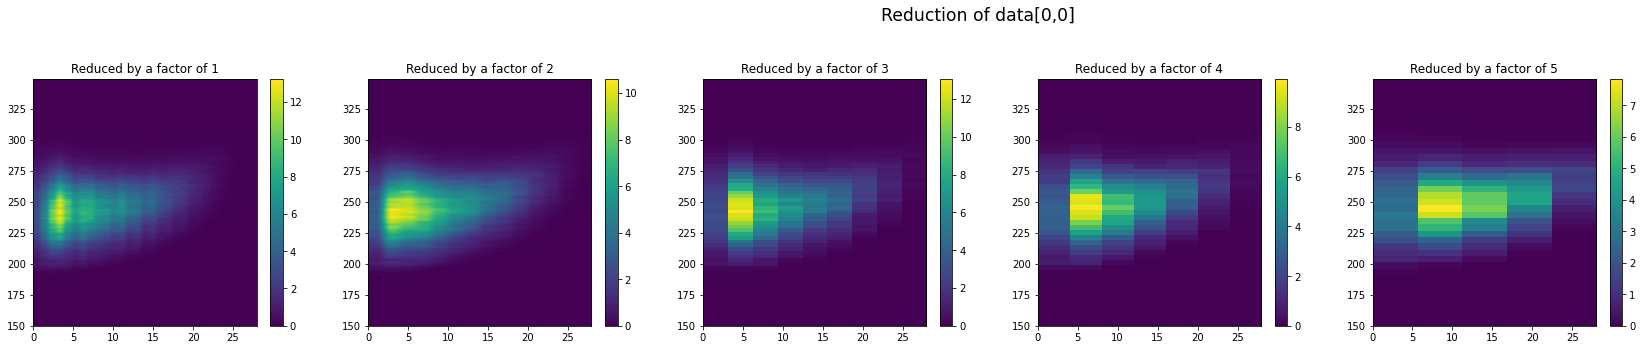
\includegraphics[width=\linewidth]{reducedHist}
	\caption{Reduced Histograms}
	\label{fig:reducedHist}
	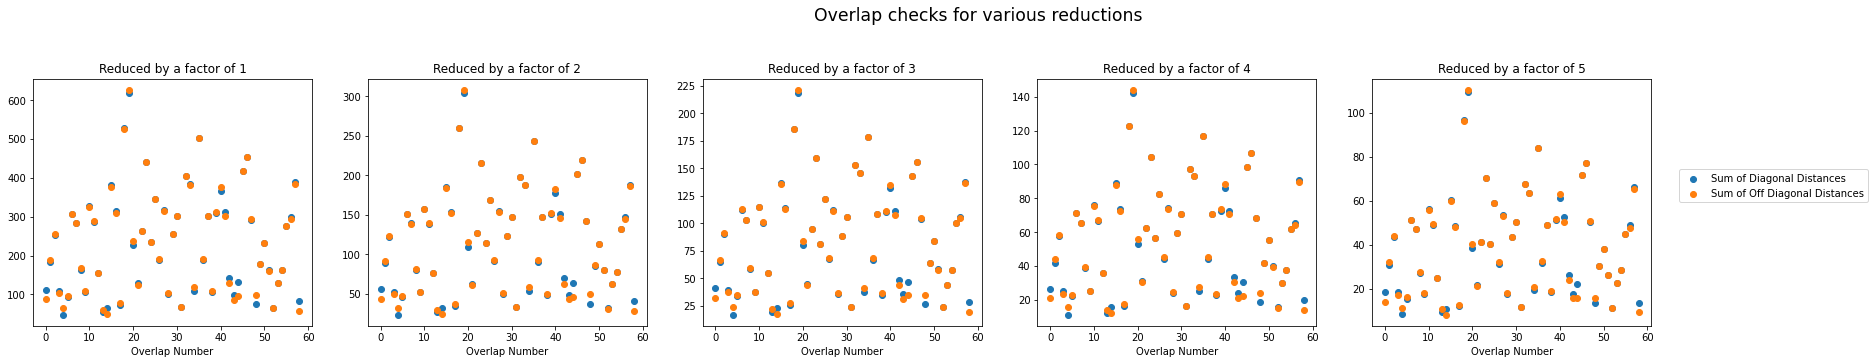
\includegraphics[width=\textwidth]{reducedGraph}
	\caption{Reduced Graphs}
	\label{fig:reducedGraph}
\end{figure}


\section{Conclusion}

\printbibliography

\end{document}
 
